\chapter{Progettazione} %------------------------------ CHAPTER TITLE
Il progetto di stage prevede lo sviluppo di vari componenti software.\\
Prima di procedere con l'implementazione, è stato dedicato del tempo alla fase di progettazione.\\
Durante questo periodo sono state prese delle decisioni importanti riguardo all'architettura e le strade da seguire. Si è cercato quindi di adottare il modo più semplice ed efficace per ottenere il risultato voluto.\\
In questo capitolo verrà illustrata la progettazione sottostante e come i componenti software sviluppati si inseriscono all'interno del sistema.\\
L'obiettivo è quello di fornire una visione globale dell'architettura adottata.
  
\thispagestyle{empty}

\newpage
\section{Architettura}
L'architettura ad alto livello che si vuole utilizzare è molto semplice. Essa prevede l'implementazione di un componente SAPI~5 e lo sviluppo di un canale di comunicazione verso un engine TTS.\\
Per facilitare lo svolgimento del progetto si è scelto di utilizzare, in congiunta con il committente, un esempio guida chiamato \gls{salbg}.\\
SALB è un progetto open source pensato per offrire tramite la specifica SAPI~5 le funzionalità di sintesi vocale ottenute dall'utilizzo congiunto di flite e delle voci basate su modelli HMM elaborate da \gls{hts}.\\
Partendo da questo progetto, andranno analizzate le varie parti che lo compongono e verranno individuate le best practice da introdurre nel progetto di stage.\\
Riassumendo, i vari componenti che verranno utilizzati sono:
\begin{description}
	\item[Interfaccia SAPI~5] interfaccia messa a disposizione dal sistema operativo Microsoft Windows che permette di implementare le funzionalità di sintesi e riconoscimento vocale;
	\item[Implementazione interfaccia SAPI~5] insieme delle funzionalità in grado di permettere la comunicazione tramite la specifica SAPI~5 tra l'engine TTS scelto e la sua destinazione, che potrà essere il sistema operativo o le applicazioni utente; 
	\item[Engine TTS] engine di sintesi vocale messo a disposizione dall'azienda, che può essere MaryTTS o Speect.
\end{description}

\subsection{Architettura engine SAPI~5 mediante MaryTTS}
L'architettura adottata per rendere fruibile l'engine MaryTTS dal sistema operativo Microsoft Windows è composta dai seguenti componenti:
\begin{description}
	\item[FATTS] implementa l'interfaccia SAPI~5 e ha il compito di dialogare con il sistema operativo Microsoft Windows e di interagire con il componente \textbf{fatts\_client}.
	\item[fatts\_client] è il componente che interagisce attraverso richieste HTTP con l'engine MaryTTS utilizzando la libreria cURL.\\
	Ogni volta che viene effettuata una richiesta all'engine, \textbf{fatts\_client} si preoccupa di gestire l'output e di trasferirlo a \textbf{FATTS}.
\end{description}

\begin{figure}[H]
	\centering
	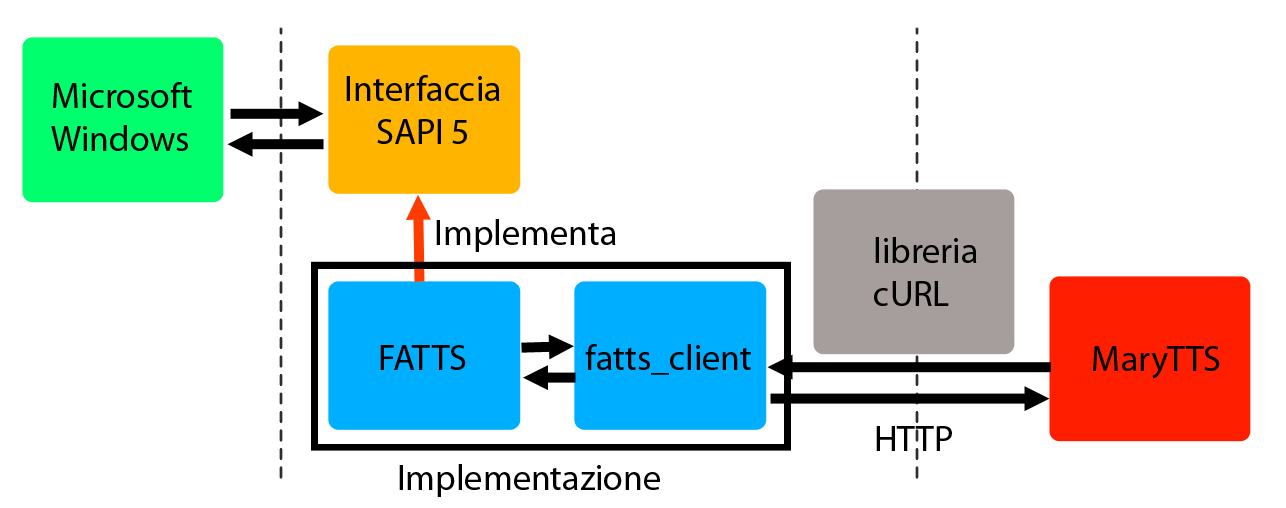
\includegraphics[width=\textwidth]{images/FATTS-sapi5.png}
	\caption{Architettura engine SAPI~5 mediante MaryTTS}
\end{figure}

\subsection{Architettura engine SAPI~5 mediante Speect}
L'architettura dell'engine SAPI~5 mediante Speect è analoga a quella ottenuta per MaryTTS ed è composta dai seguenti componenti: 
\begin{description}
	\item[SpeectTTS] implementa l'interfaccia SAPI~5 e ha il compito di dialogare con il sistema operativo Microsoft Windows e di interagire con il componente \textbf{audio\_event\_functions}.
	\item[audio\_event\_functions] è il componente che interagisce mediante chiamate a funzioni C con Speect, gestisce l'output e lo ridirige verso \textbf{SpeectTTS}. 
\end{description}

\begin{figure}[H]
	\centering
	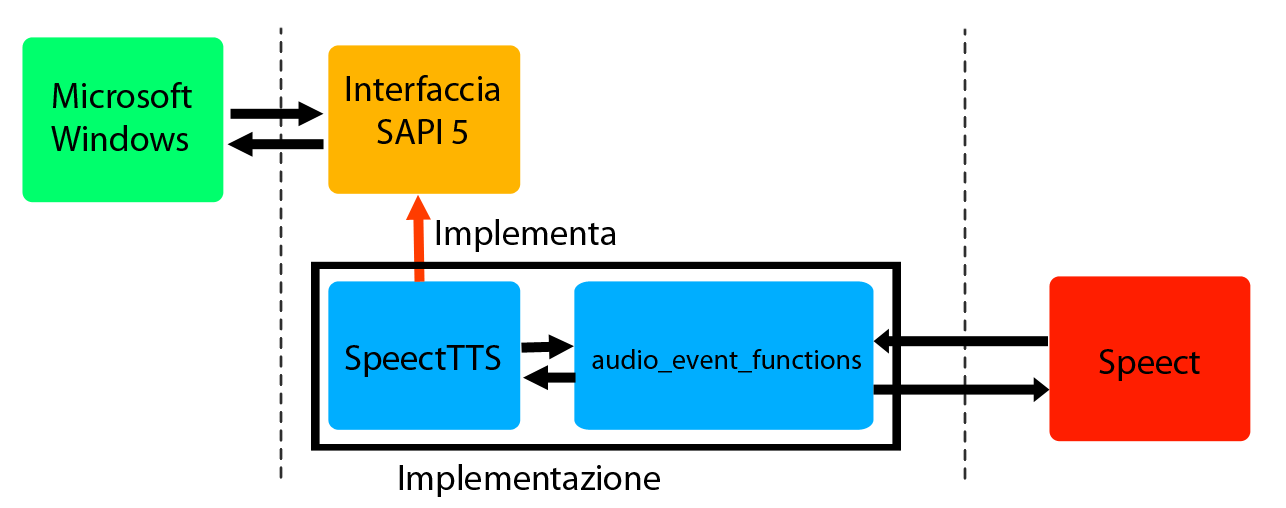
\includegraphics[width=\textwidth]{images/SpeectTTS-sapi5.png}
	\caption{Architettura engine SAPI~5 mediante SpeectTTS}
\end{figure}

I componenti sopraelencati verranno descritti in dettaglio nel capitolo \hyperref[chap:descrizione-dei-componenti]{Descrizione dei Componenti}.
	
	